%% =============================================================
%%  Les ornements — de l'appogiature à la fioriture
%%  Guide de référence, composé en LaTeX, gravures LilyPond
%% =============================================================
%%
%%  Les figures (gravures/o-*.cropped.pdf), les réponses de l'exercice
%%  (gravures/ornements-reponses.tex) et le fichier ornements.musicxml
%%  sont produits par outils/generer_ornements.py, à partir du modèle
%%  de hauteurs des autres guides (outils/gammes.py). Voir le colophon
%%  en dernière page.
%%
\documentclass[a4paper,11pt]{article}

\usepackage[top=2.2cm,bottom=2.4cm,left=2.2cm,right=2.2cm]{geometry}
\usepackage[T1]{fontenc}
\usepackage[utf8]{inputenc}
\usepackage[french]{babel}
\usepackage{lmodern}
\usepackage{xcolor}
\usepackage{graphicx}
\usepackage{titlesec}
\usepackage{fancyhdr}
\usepackage{booktabs}
\usepackage{array}
\usepackage{mdframed}
\usepackage{enumitem}
\usepackage{hyperref}

\graphicspath{{gravures/}}

% ---- Couleurs, reprises du document des accords de guitare ---------
\definecolor{navy}{RGB}{18,50,105}
\definecolor{lightnavy}{RGB}{235,241,255}
\definecolor{mygray}{RGB}{110,110,110}

\hypersetup{colorlinks=true, linkcolor=navy, urlcolor=navy,
  pdftitle={Les ornements — de l'appogiature à la fioriture},
  pdfauthor={Fabian Bastin}}

% ---- En-tête et pied -----------------------------------------------
\pagestyle{fancy}
\fancyhf{}
\renewcommand{\headrulewidth}{0.4pt}
\renewcommand{\footrulewidth}{0.4pt}
\fancyhead[L]{\small\bfseries\textcolor{navy}{Les ornements}}
\fancyhead[R]{\small\textcolor{mygray}{\thepage}}
\fancyfoot[C]{\small\textcolor{mygray}{De l'appogiature à la fioriture}}

% ---- Titres de section ---------------------------------------------
\newcommand{\navysect}[1]{%
  \colorbox{navy}{%
    \parbox[c][17pt]{\dimexpr\linewidth-2\fboxsep\relax}{%
      \color{white}\hspace{6pt}\bfseries\normalsize #1}}%
}
\titleformat{\section}[block]{\normalfont}{}{0pt}{\navysect}
\titlespacing*{\section}{0pt}{16pt}{10pt}

% ---- Encadré de remarque -------------------------------------------
\newmdenv[linecolor=navy, linewidth=0.5pt, backgroundcolor=lightnavy,
  innertopmargin=6pt, innerbottommargin=6pt,
  innerleftmargin=8pt, innerrightmargin=8pt,
  skipabove=8pt, skipbelow=8pt]{remarque}

% ---- Figure gravée ---------------------------------------------------
% Figure gravée, à la largeur donnée (part de la ligne), avec sa légende.
% Le tout tient dans une minipage : figure et légende ne sont jamais
% séparées par un saut de page. Les largeurs suivent la largeur naturelle
% des gravures, pour que toutes aient la même échelle.
\newcommand{\gravure}[3]{%
  \par\medskip\noindent
  \begin{minipage}{\linewidth}
    \centering
    \includegraphics[width=#2\linewidth]{#1.cropped.pdf}\\[4pt]
    {\small\itshape\color{mygray} #3}
  \end{minipage}\par\medskip
}

% Siècle en petites capitales, droites même dans une légende en italique.
\newcommand{\siecle}[1]{{\upshape\textsc{#1}}\textsuperscript{e}~siècle}

\setlist{itemsep=2pt, topsep=4pt, parsep=0pt}

\begin{document}

% =====================================================================
\begin{titlepage}
\centering
\vspace*{3cm}
{\Huge\bfseries\color{navy} Les ornements\par}
\vspace{0.6cm}
{\LARGE\color{navy} De l'appogiature à la fioriture\par}
\vspace{1.4cm}
{\large Petites notes et signes, et ce qu'ils font jouer\par}
\vspace{2.5cm}
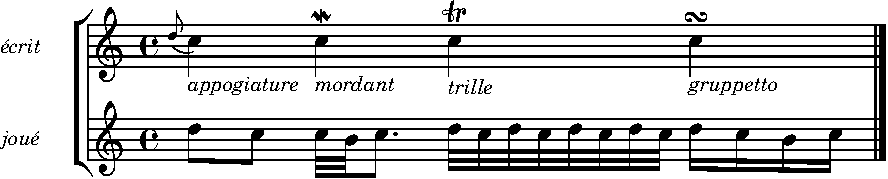
\includegraphics[width=0.85\linewidth]{o-apercu.cropped.pdf}
\vfill
{\small\color{mygray}
Gravures LilyPond, composition \LaTeX.\\
Fichier MusicXML joint.\par}
\vspace{1cm}
\end{titlepage}

\tableofcontents
\newpage

% =====================================================================
\section{Avant-propos}

Un \textbf{ornement} ajoute à une note des notes brèves qui l'embellissent
sans changer le dessin de la mélodie ; les clavecinistes français disaient
\emph{agrément}. Il s'écrit en petites notes ou par un signe, et ce qu'il faut
jouer se déduit de règles. Au programme de matières théoriques de l'École de
musique Vincent-d'Indy, ces notions relèvent des niveaux 3 et 5.

À lire après
\href{https://www.slashbin.net/musique/theorie/lecture.pdf}{\emph{Lire les
notes}}, \href{https://www.slashbin.net/musique/theorie/valeurs.pdf}{\emph{Les valeurs}} et
\href{https://www.slashbin.net/musique/theorie/intervalles.pdf}{\emph{Les
intervalles}} : un ornement se mesure en valeurs de notes, et l'écart entre une
note et ses voisines en tons et en demi-tons. Le mordant a son propre guide,
\href{https://www.slashbin.net/musique/theorie/mordants.pdf}{\emph{Les
mordants}}.

\begin{remarque}
\textbf{Conventions.} Les notes sont nommées en français. La \emph{note
principale} est la note ornée ; ses \emph{voisines}, les notes immédiatement
au-dessus et au-dessous d'elle dans la gamme. Les exemples sont en clé de sol
et, sauf mention contraire, en do majeur ; chaque gravure montre en haut ce qui
est écrit, en bas ce qui est joué. Les notes jouées y sont mesurées à la
noire 80 : les plus vives en triples croches, un peu moins d'un dixième de
seconde chacune, celles du gruppetto sur la note en doubles croches. Ces valeurs sont une
commodité d'écriture ; l'allure réelle dépend du tempo, de l'instrument et du
goût.
\end{remarque}

Le fichier MusicXML joint fait entendre chaque exemple ; la
section~\ref{sec:musicxml} le présente.

% =====================================================================
\section{Petites notes et signes}
\label{sec:ecritures}

\textbf{Les petites notes.} Gravées en petit caractère devant la note
principale, ou après elle, elles ne comptent pas dans la mesure : le temps
qu'elles prennent est pris à une note voisine, le plus souvent à la note
principale. L'appogiature, l'appogiature brève et la fioriture s'écrivent
ainsi, comme la terminaison du trille.

\textbf{Les signes.} Au-dessus de la note, un signe désigne un motif : le
mordant, le trille, le gruppetto. Il ne dit pas les notes elles-mêmes : les
voisines se prennent dans la gamme que désigne l'armure, sauf altération
écrite près du signe.

\textbf{Sur le temps.} Dans la musique baroque et classique, un ornement
commence le plus souvent sur le temps de la note qu'il orne et lui prend son
temps : c'est la note principale qui arrive en retard, non la précédente qui
raccourcit. Le \siecle{xix} assouplit la règle pour l'appogiature brève et la
fioriture.

\gravure{o-apercu}{1}{L'appogiature, le mordant, le trille et le gruppetto sur
do, écrits en haut, joués en bas. Chacun commence sur le temps et tient dans la
valeur de sa note.}

% =====================================================================
\section{L'appogiature}
\label{sec:appogiature}

\textbf{La note sur laquelle on s'appuie.} L'appogiature est une petite note,
sans trait, écrite devant la note principale, presque toujours une seconde
au-dessus ou au-dessous d'elle. Son nom vient de l'italien \emph{appoggiare},
appuyer : elle tombe sur le temps, à la place de la note principale, qui
n'arrive qu'ensuite. Souvent étrangère à l'harmonie, elle crée une tension que
la note principale résout ; on appuie l'appogiature, on allège la note qui la
suit.

\textbf{La moitié de la note.} Devant une note simple, l'appogiature en prend
la moitié. C.~P.~E. Bach en fait la règle générale dans son \emph{Essai sur la
vraie manière de jouer des instruments à clavier} (1753) ; elle vaut sur toute
valeur : une noire devant une blanche, une croche devant une noire, une double
croche devant une croche.

\gravure{o-appogiature}{0.84}{L'appogiature prend la moitié d'une blanche,
d'une noire, d'une croche. Elle vient d'en haut ou d'en bas.}

\textbf{La valeur gravée ne fait pas foi.} Les gravures écrivent toutes les
appogiatures en petites croches, comme les éditions anciennes : C.~P.~E. Bach
rapporte qu'on les notait autrefois ainsi, quelle que fût leur durée, et que
de son temps on commençait à les écrire à leur valeur réelle. Au
\siecle{xix}, les compositeurs les écrivent de plus en plus en notes
ordinaires, à leur place dans la mesure. Devant une petite note, c'est donc la
règle qui donne la durée ; la valeur gravée ne la donne que si l'édition l'a
voulue exacte.

\textbf{Les deux tiers d'une note pointée.} Devant une note pointée,
l'appogiature en prend les deux tiers --- une blanche devant une blanche
pointée, une noire devant une noire pointée ---, et la note principale ne garde
que la valeur du point. C'est la seconde moitié de la règle de C.~P.~E. Bach.

\textbf{Toute la note devant un silence.} Quand la note principale est suivie
d'un silence, l'appogiature peut prendre toute sa valeur ; la note principale
se joue alors à la place du silence. Quantz, C.~P.~E. Bach et Leopold Mozart
le décrivent ; le phrasé, et pour un chanteur la respiration, en décident.

\gravure{o-appog-longues}{0.66}{Sur une blanche pointée et sur une noire
pointée, l'appogiature prend les deux tiers de la note ; devant un silence,
toute la note, et do se joue à la place du silence.}

\begin{remarque}
\textbf{Le port de voix.} Les clavecinistes français appelaient \emph{port de
voix} l'appogiature venue d'en bas, souvent suivie d'un \emph{pincé}, leur nom
du mordant.
\end{remarque}

% =====================================================================
\section{L'appogiature brève}
\label{sec:breve}

\textbf{Une petite note barrée.} L'appogiature brève s'écrit en petite croche
dont la hampe et le crochet sont traversés d'un trait oblique. On l'appelle
aussi \emph{acciaccatura}, de l'italien \emph{acciaccare}, écraser : elle
s'écrase contre la note principale, qui reçoit l'accent.

\textbf{Aussi brève sur toute valeur.} Elle passe aussi vite que possible et
ne prend presque rien à la note principale, quelle que soit sa valeur, même
dans un mouvement lent : une triple croche dans les gravures, sur une noire
comme sur une blanche. C.~P.~E. Bach distinguait déjà ces appogiatures
invariables, toujours brèves, des appogiatures longues, dont la durée suit la
note ; il les écrivait avec un, deux crochets ou davantage. Le trait ne s'impose
qu'au \siecle{xix}.

\gravure{o-acciaccatura}{0.75}{La même petite note devant do, longue puis
brève : la moitié de la noire, puis une triple croche. Brève, elle ne prend pas
davantage à une blanche.}

\begin{remarque}
\textbf{Sur le temps, ou juste avant.} Au \siecle{xviii} déjà, les auteurs ne
s'accordent pas : les uns placent l'appogiature brève sur le temps, d'autres,
comme Quantz, juste avant. Au \siecle{xix}, on la place souvent avant le temps,
pour que la note principale tombe avec la basse. Les gravures la placent sur le
temps ; le style et le contexte décident. Au début du \siecle{xviii}, en
Italie, le mot \emph{acciaccatura} désignait encore autre chose : une note
étrangère frappée avec un accord et aussitôt relâchée.
\end{remarque}

% =====================================================================
\section{Le mordant}
\label{sec:mordant}

Le mordant s'écrit par un court zigzag barré d'un trait vertical. Il fait
entendre la note principale, sa voisine du dessous, puis de nouveau la note :
les deux premières très vite et sur le temps, la dernière tenue jusqu'au bout
de la valeur. Sans le trait, le même zigzag désigne aujourd'hui le mordant
supérieur, avec la voisine du dessus ; chez Bach, c'était un trille court. Ses
règles, ses noms et ses deux lectures sont l'objet de
\href{https://www.slashbin.net/musique/theorie/mordants.pdf}{\emph{Les
mordants}}.

% =====================================================================
\section{Le trille}
\label{sec:trille}

\textbf{Le signe.} Le trille s'écrit \emph{tr} au-dessus de la note, souvent
suivi d'une ligne ondulée qui en couvre la durée. Les clavecinistes français
l'appelaient \emph{tremblement} ou \emph{cadence} : c'est à la cadence, sur la
sensible, qu'on l'entend le plus.

\textbf{L'alternance.} Le trille alterne rapidement la note principale et sa
voisine du dessus, prise dans la gamme, jusqu'au bout de la valeur. Une
altération écrite près du signe change cette voisine : sur ré, en do majeur,
\emph{tr} accompagné d'un bémol fait alterner ré et mi bémol. Le nombre de
notes ne se compte pas, il dépend du tempo et de la longueur de la note ; à la
noire 80, les gravures en mettent huit par noire.

\textbf{La terminaison.} Un trille sur une note longue s'achève par une
\emph{terminaison} : la voisine du dessous, puis la note, qui mènent à la note
suivante. Elle s'écrit en deux petites notes après la note trillée.
C.~P.~E. Bach la nomme \emph{Nachschlag} et la juge de rigueur sur un trille
assez long, même quand rien ne l'indique.

\gravure{o-trille}{0.96}{Un trille long sur si, avec la ligne ondulée et la
terminaison écrite en petites notes : l'alternance, commencée sur la voisine
comme au \siecle{xviii}, puis la et si, et do à la mesure suivante.}

\textbf{La note de départ.} Au \siecle{xviii}, le trille commence sur la
voisine du dessus, sur le temps : C.~P.~E. Bach écrit qu'il commence toujours
par la note au-dessus de la note principale, et Leopold Mozart l'enseigne de
même au violon. Cette première note sonne comme une brève appogiature. Au
\siecle{xix}, le trille commence le plus souvent sur la note elle-même ; la
méthode de piano de Hummel, en 1828, ne donne plus que cette manière.

\gravure{o-trille-epoques}{0.62}{Le trille sur si, la sensible de do majeur,
lu à deux époques : au \siecle{xviii}, commencé sur la voisine, do ; au
\siecle{xix}, sur la note. Dans les deux cas, il s'achève sur si.}

\begin{remarque}
\textbf{Entre les deux époques.} Pour la musique de la fin du
\siecle{xviii} --- Haydn, Mozart, Beethoven ---, les interprètes et les
éditeurs ne s'accordent pas toujours. Une petite note écrite devant le trille
tranche la question : elle en donne la première note.
\end{remarque}

% =====================================================================
\section{Le gruppetto}
\label{sec:gruppetto}

\textbf{Le signe et ses quatre notes.} Le gruppetto s'écrit par un S couché.
Son nom italien veut dire petit groupe : la voisine du dessus, la note, la
voisine du dessous, la note. Il fait le tour de la note.

\textbf{Sur la note.} Placé au-dessus de la note, il commence sur le temps :
les trois premières notes passent vite, la dernière est tenue jusqu'au bout de
la valeur. Les gravures l'écrivent en doubles croches.

\textbf{Après la note.} Placé entre une note et la suivante, il s'entend à la
fin de la note : on tient d'abord la note, puis le tour mène à la suivante. Les
gravures donnent à la note la moitié de sa valeur, et au tour l'autre moitié ;
c'est une lecture parmi d'autres, car le rythme du gruppetto varie avec le
tempo et le goût.

\textbf{Renversé.} Retourné, ou barré d'un trait vertical, le signe désigne le
\emph{gruppetto renversé}, qui commence par en bas : la voisine du dessous, la
note, la voisine du dessus, la note.

\gravure{o-gruppetto}{0.91}{Le gruppetto sur do : au-dessus de la note, puis
après elle, puis renversé.}

\textbf{Les altérations.} Le gruppetto emploie les deux voisines. Une
altération près du signe change celle de son côté : au-dessus du signe pour la
voisine du dessus, au-dessous pour la voisine du dessous.

\gravure{o-gruppetto-alt}{0.52}{Le gruppetto sur sol, en do majeur : la voisine
du dessous est fa ; avec un dièse sous le signe, fa dièse.}

% =====================================================================
\section{La fioriture}
\label{sec:fioriture}

\textbf{Un passage libre.} Une \emph{fioriture} --- de l'italien
\emph{fioritura}, floraison --- est une suite de petites notes, parfois
longue, qui brode autour de la mélodie : fragment de gamme, arpège, broderie.
Elle vient du chant italien, où les chanteurs ornaient d'eux-mêmes la reprise
d'un air ; au \siecle{xix}, Chopin en orne ses nocturnes, à l'image du
\emph{bel canto} de Bellini.

\textbf{Un rythme libre.} Les petites notes d'une fioriture ne se comptent
pas : l'interprète les place avec souplesse, et la mélodie retrouve ensuite sa
mesure. La gravure en donne une lecture parmi d'autres : la fioriture prend son
temps à la fin de la note qui la précède, et la note qui la suit tombe à sa
place.

\gravure{o-fioriture}{0.85}{Une fioriture de huit petites notes entre mi et
fa, jouée ici pendant le second temps de mi.}

% =====================================================================
\section{Les ornements en un tableau}
\label{sec:tableau}

\begin{center}
\small
\renewcommand{\arraystretch}{1.25}
\begin{tabular}{@{}>{\raggedright}p{0.2\linewidth}>{\raggedright}p{0.2\linewidth}
                >{\raggedright}p{0.3\linewidth}>{\raggedright\arraybackslash}p{0.2\linewidth}@{}}
\toprule
\textbf{Ornement} & \textbf{Écriture} & \textbf{Sur do, en do majeur} & \textbf{Place} \\
\midrule
appogiature & petite note & ré, puis do : la moitié de la note, les deux
  tiers si elle est pointée & sur le temps \\
appogiature brève & petite note barrée & ré très bref, puis do & sur le temps,
  ou juste avant \\
mordant & zigzag barré & do, si, do & sur le temps \\
trille & \emph{tr}, ligne ondulée & ré, do, ré, do\ldots{} ou do, ré, do,
  ré\ldots{} jusqu'au bout de la note & sur le temps \\
gruppetto & S couché & ré, do, si, do & sur la note, ou après elle \\
gruppetto renversé & S retourné ou barré & si, do, ré, do & sur la note, ou
  après elle \\
fioriture & petites notes & libres & rythme libre \\
\bottomrule
\end{tabular}
\end{center}

% =====================================================================
\section{S'exercer}
\label{sec:exercices}

Pour chaque ornement numéroté, le nommer et donner les notes jouées avec leurs
valeurs, selon les conventions des gravures : triples croches pour les notes
vives, doubles croches pour le gruppetto. Le trille commence sur la voisine,
comme au \siecle{xviii}, et l'appogiature brève sur le temps. Les réponses
suivent.

\gravure{o-exercice}{0.62}{Une mélodie en fa majeur, à trois temps.}

\begin{remarque}
\textbf{Réponses.}
%% Produit par outils/generer_ornements.py — ne pas modifier à la main.
\begin{enumerate}[label=\textbf{\arabic*}~:, leftmargin=2.2em, itemsep=1pt]
  \item appogiature --- ré (blanche), do (noire).
  \item gruppetto après la note --- la (noire), si bémol, la, sol, la (doubles croches).
  \item mordant --- si bémol, la (triples croches), si bémol (croche pointée).
  \item appogiature brève --- la (triple croche), sol (croche doublement pointée).
  \item gruppetto --- ré, do, si bémol, do (doubles croches).
  \item appogiature --- sol, fa (croches).
  \item trille avec terminaison --- fa et mi sept fois, puis ré, mi (triples croches).
\end{enumerate}

\end{remarque}

% =====================================================================
\section{Le fichier MusicXML}
\label{sec:musicxml}

Le fichier joint, \texttt{ornements.musicxml}, reprend chaque gravure, puis la
mélodie de l'exercice, écrites en toutes notes telles qu'elles se jouent, à la
noire 80 ; le trille sur si y figure sous ses deux lectures. Les petites notes
et les signes n'y figurent pas : tout logiciel fait ainsi entendre la même
chose. Il se lit avec MuseScore, Finale, Sibelius, Dorico ou tout éditeur de
partitions ; sur slashbin.net, il s'écoute aussi dans Sodor Piano.

% =====================================================================
\section*{Colophon}
\addcontentsline{toc}{section}{Colophon}

Les gravures musicales sont produites par \textbf{LilyPond}, la composition
par \textbf{\LaTeX}. Les portées jouées, les réponses de l'exercice et le
fichier MusicXML dérivent du modèle de hauteurs des autres guides, le module
\texttt{gammes.py} du dossier \texttt{outils}, et d'une règle par ornement,
celle du mordant et du gruppetto étant partagée avec \emph{Les mordants}.
Avant d'écrire quoi que ce soit, le générateur vérifie ce que le texte
affirme : la moitié et les deux tiers de l'appogiature, la même triple croche
pour l'appogiature brève sur toute valeur, le trille achevé sur la note à
chaque époque, les voisines prises dans la gamme ou changées par l'altération
écrite, chaque mesure jouée complète. Pour régénérer l'ensemble :

\begin{center}
\texttt{python3 outils/generer\_ornements.py}\\
\texttt{(cd gravures \&\& lilypond -dcrop --formats=pdf o-*.ly)}\\
\texttt{pdflatex ornements.tex}
\end{center}

\end{document}
